\chapter{Verification Dataset}
\label{chapter:vds}


\section{Overview}

\begin{table}
\caption{ \smr\ VDS content.}
\label{table:comp}
\begin{tabular}{|l|l|l|}
\hline
\textbf{Frequency mode} & \textbf{Instrument} &  \textbf{Species}\\
\hline
    1  &     SMILES   &      \chem{O_3} \\
       &     MLS      &      \chem{O_3}, \chem{ClO}, \chem{N_{2}O} \\
       &     MIPAS    &      \chem{O_3}, \chem{N_{2}O} \\
       &     SAGEIII  &      \chem{O_3} \\
\hline
    2  &     SMILES   &      \chem{O_3}, \chem{HNO_3} \\
       &     MLS      &      \chem{O_3}, \chem{HNO_3} \\
       &     MIPAS    &      \chem{O_3}, \chem{HNO_3} \\
       &     SAGEIII  &      \chem{O_3} \\
\hline
    8  &     SMILES   &      \chem{O_3} \\
       &     MLS      &      \chem{O_3}, \chem{H_{2}O} \\
       &     MIPAS    &      \chem{O_3}, \chem{H_{2}O} \\
       &     SAGEIII  &      \chem{O_3} \\
\hline
   13  &     SMILES   &      \chem{O_3} \\
       &     MLS      &      \chem{O_3}, \chem{H_{2}O} \\
       &     MIPAS    &      \chem{O_3}, \chem{H_{2}O} \\
       &     SAGEIII  &      \chem{O_3} \\
\hline
   17  &     SMILES   &      \chem{O_3} \\
       &     MLS      &      \chem{O_3}, \chem{H_{2}O} \\
       &     MIPAS    &      \chem{O_3}, \chem{H_{2}O} \\
       &     SAGEIII  &      \chem{O_3} \\
\hline
   19  &     SMILES   &      \chem{O_3} \\
       &     MLS      &      \chem{O_3}, \chem{H_{2}O} \\
       &     MIPAS    &      \chem{O_3}, \chem{H_{2}O} \\
       &     SAGEIII  &      \chem{O_3} \\
\hline
   21  &     SMILES   &      \chem{O_3}, \chem{NO} \\
       &     MLS      &      \chem{O_3}, \chem{H_{2}O} \\
       &     MIPAS    &      \chem{O_3}, \chem{H_{2}O} \\
       &     SAGEIII  &      \chem{O_3} \\
\hline
\end{tabular}
\end{table}


The verfication dataset (VDS) consists of a represenative subset of 
the \smr\ complete dataset, and correlative datasets.
In short, the VDS is a dateset of \smr\ measurements 
and collocated measurements from a number of correlative
limb-sounding instruments. 
Table~\ref{table:comp} gives an overview of the correlative
datasets included in the VDS, and these datasets
are, in more details, described in Sect.~\ref{sec:corrmeas}.
Sect.~\ref{sec:vdsselection} describes collocation criterias
applied and how the VDS was selected. 
    

\clearpage
\newpage

\section{Correlative measurements}
\label{sec:corrmeas}
\subsection{Aura/MLS}

The Aura satellite was launched on 2004-07-15 into a 
sun-synchronous orbit at 705\,km altitude, with an ascending
equator crossing local time of 13:45. Its
orbit is near-polar with a 98\degree inclination, 
and the daily Microwave Limb Sounder (MLS) measurements cover 
the latitudinal range from about 82\degree\,S to 82\degree\,N. 
MLS measures temperature and trace gas profiles 
using thermal emission data from the
upper troposphere to the mesosphere. MLS performs each
limb scan and related calibration in 25\,s, and 
obtains \(\sim\) 3500 vertical profiles a day 
\citep{waters:eos:06}. The MLS data
processing algorithms are based on the optimal estimation
method (OEM), as explained by \citet{livesey:MLS}. MLS uses
spectral bands centered near 118, 190, 240, 640\,GHz,
and 2.3\,THz. 

The Aura/MLS Level2 products, and characteristics, included in the
VDS are found in Table~\ref{table:mlslevel2}.


\begin{table}
\caption{ Characteristics of Aura/MLS Level2 data products included in the VDS.
Considered Level2 version is v04-20.}
\label{table:mlslevel2}
\begin{tabular}{|l|l|l|l|l|l|}
  \hline
  \textbf{Product}      & \textbf{Vertical}          & \textbf{Vertical}            & \textbf{Precision} & \textbf{Reference}   \\
                        & \textbf{coverage}          & \textbf{resolution}          &                    &                      \\
  \hline
  \chem{O_{3}}          & 261--0.02\,hPa             &  3.5--5.5\,km                & 0.03--1.2\,ppmv    &  \citep{livesey:MLS} \\
  \hline
  \chem{ClO}            & 147--1.0\,hPa              &  3--4.5\,km                  & 0.1--0.3\,ppbv     &  \citep{livesey:MLS} \\
  \hline
  \chem{N_{2}O}         & 68--0.46\,hPa              &  5.4--11\,km                 & \(\sim\)15\,ppbv   &  \citep{livesey:MLS} \\
  \hline
  \chem{HNO_{3}}        & 215--1.5\,hPa              &  4--4.5\,km                  & 1--0.5\,ppbv       &  \citep{livesey:MLS} \\
  \hline
  \chem{H_{2}O}         & 316--0.002\,hPa            &  1.3--10\,km                 & 4--152\,\(\%\)     &  \citep{livesey:MLS} \\
  \hline   

\end{tabular}
\end{table}




\subsection{ENVISAT/MIPAS}

The Michelson Interferometer for Passive Atmospheric
Sounding (MIPAS) is a mid-infrared emission spectrometer
mounted on the European ENVIronmantal SATellite (ENVISAT),
which was launched in 2002-03-01 \citep{fischer2008},
and was in operation until 2012-04-08. 
ENVISAT has a sun-synchronous orbit at an altitude of 800\,km
and with a 98.55\degree inclination and descending equator 
crossing local time of 10:00.

The failure of a MIPAS mirror slide in 2004 led to the 
division of the 10 years of MIPAS
data into two operational periods: 2002--2004 when the 
instrument measured with high spectral resolution 
and 2005--2012 when the instrument measured with lower 
spectral but better vertical resolution.

MIPAS observed five mid-infrared spectral bands within the
frequency range of 685 to 2410\,cm\(^{-1}\) (14.6 to 4.15\,\(\mu\)m),
with a resolution of 0.0625\,cm\(^{-1}\).
Until 2004-03-26 MIPAS scanned 17 tangent altitudes from 
6 to 68\,km with 3,-\,8\,km resolution.
From January 2005 MIPAS started operating in a new mode
at a reduced spectral resolution but at a finer altitude
grid. The latitudinal coverage was from 87\degree\,S to 89\degree\,N.
In the latter mode, MIPAS had about 95 scans per orbit, and about
1360 vertical profiles were recorded in a day.

Opertaional Level-2 data from MIPAS is generated by ESA,
but we here consider the MIPAS scientific data product
generated by the Institut fur Meteorologie und Klimatforscung
(IMK) at Karlsruhe Institude of Technology (KIT).

The  ENVISAT/MIPAS Level2 products and characteristics included in the
VDS are found in Table~\ref{table:mipaslevel2}.

% O3 - 200207.V5H_O3_21.nc --  MIPAS-E_IMK.200501.V5R_O3_224.nc -- MIPAS-E_IMK.201106.V5R_O3_225.nc 
% MIPAS-E_IMK.200207.V5H_N2O_21.nc --  MIPAS-E_IMK.200501.V5R_N2O_224.nc --  MIPAS-E_IMK.201106.V5R_N2O_225.nc
% MIPAS-E_IMK.200207.V5H_HNO3_22.nc -- MIPAS-E_IMK.200501.V5R_HNO3_224.nc --  MIPAS-E_IMK.201106.V5R_HNO3_225.nc 
% MIPAS-E_IMK.200207.V5H_H2O_20.nc --  MIPAS-E_IMK.200506.V5R_H2O_220.nc  -- MIPAS-E_IMK.201106.V5R_H2O_221.nc

% o3: http://www.atmos-meas-tech.net/7/3971/2014/amt-7-3971-2014.pdf
% http://www.atmos-chem-phys.net/7/3639/2007/acp-7-3639-2007.pdf

\begin{table}
\caption{ Characteristics of ENVISAT/MIPAS Level2 data products included in the VDS.}
\label{table:mipaslevel2}
\begin{tabular}{|l|l|l|l|l|l|l|}
  \hline
  \textbf{Product}      & \textbf{Vertical}          & \textbf{Vertical}            & \textbf{Precision} &  \textbf{Version}    & \textbf{Reference} \\
                        & \textbf{coverage}          & \textbf{resolution}          &                    &                      &                    \\
  \hline
  \chem{O_{3}}          & \(\sim\)10--60\,km         &  3.5 -- 8\,km                & 0.1--0.2\,ppmv     &  V5H-O3-21           &  Steck et al 2007\\
                        &                            &                              &                    &  2002-07 -- 2004-03  &   \\ 
  \hline
  \chem{O_{3}}          & \(\sim\)10--70\,km         &  2 -- 6\,km                  & 0.03--0.09\,ppmv   &  V5R-O3-22(4/5)      &  Laeng et al 2014\\
                        &                            &                              &                    &  2005-01 -- 2012-04  &   \\
  \hline 
  \chem{N_{2}O}         & \(\sim\)15--70\,km         &  ?\,km                       & 15--35\,ppbv       &  V5H-N2O-21          &  ?\\
                        &                            &                              &                    &  2002-07 -- 2004-03  &   \\
  \hline
  \chem{N_{2}O}         & \(\sim\)15--70\,km         &  ?\,km                       & 15--35\,ppbv       &  V5R-N2O-22(4/5)     &  ?\\
                        &                            &                              &                    &  2005-01 -- 2012-04  &   \\
  \hline
  \chem{HNO_{3}}        & \(\sim\)21--67\,km         &  ?\,km                       & 1 ppbv             &  V5H-HNO3-22         &  ?\\
                        &                            &                              &                    &  2002-07 -- 2004-03  &   \\
  \hline
  \chem{HNO_{3}}        & \(\sim\)21--67\,km         &  ?\,km                       & 1 ppbv             &  V5R-HNO3-22(4/5)    &  ?\\
                        &                            &                              &                    &  2005-01 -- 2012-04  &   \\
  \hline
  \chem{H_{2}O}         & \(\sim\)21--67\,km         &  ?\,km                       & 1 ppbv             &  V5H-H2O-20          &  ?\\
                        &                            &                              &                    &  2002-07 -- 2004-03  &   \\
  \hline
  \chem{H_{2}O}         & \(\sim\)21--67\,km         &  ?\,km                       & 1 ppbv             &  V5H-H2O-22(0/1)     &  ?\\
                        &                            &                              &                    &  2005-01 -- 2012-04  &   \\

  \hline
  


\end{tabular}
\end{table}



\subsection{ISS/JEM/SMILES}

The Superconducting Submillimeter-Wave Limb-Emission Sounder (SMILES),
attached to the Exposed Facility of the Japanese Experiment Module (JEM), 
on the International Space Station (ISS), is a joint project of the
National Institute of Information and Communications Technology (NICT) and
the Japan Aerospace Exploration Agency (JAXA).

SMILES, carried by ISS, collected thermal emission
between 2009-10-12 and 2010-04-21.
The ISS has a non-sun-synchronous circular orbit at
altitudes of 340\,-\,360\,km with an inclination angle of 51.6\degree
to the equator. The nominal latitude coverage of SMILES is from 38\degree\,S
to 65\degree\,N.

SMILES observed a number  
of trace gases, e.g.: \chem{O_{3}}, \chem{H^{35}Cl}, \chem{H^{37}Cl}, 
\chem{ClO}, \chem{HOCl}, \chem{HO_{2}}, \chem{BrO}, and \chem{HNO_{3}}, 
from the upper troposphere up to the lower thermosphere,  
between 2009-10-12 and 2010-04-21, and with a nominal latitudinal coverage 
from 38\degree\,S to 65\degree\,N.

SMILES collected atmospheric thermal emission in two frequency
bands around 625\,GHz and one around 650\,GHz;
624.32\,-\,625.52\,GHz (Band-A), 625.12\,-\,626.32\,GHz (Band-B),
and 649.12\,-\,650.32\,GHz (Band-C), with a frequency resolution
and channel separation of about 1\,MHz and 0.8\,MHz, 
respectively.  
During each measurement, two out of the three SMILES frequency
bands were observed simultaneously, by two acousto optical spectrometers,
and with a receiver noise temperature of 310\,-\,350\,K.

SMILES performed 1630 scans per day, where the limb was scanned
from about -20\,km to 120\,km (geometric altitude), 
with a sampling interval of about 2\,km, and with an angle of 
about 45\degree from the orbital plane. The size of the antenna beam, 
at the tangent point, was about 3 and 6\,km in the vertical and 
horizontal direction, respectively. 

An interesting feature of SMILES observation is related to the fact
that ISS has a non-sunsynchronous orbit, which gives that SMILES 
observations cover different local times and thereby provides insight
of the diurnal variation of atmospheric short-lived species
(e.g \chem{ClO}, \chem{BrO}, \chem{HO_2}, and \chem{HOCl}). 
A two month period is required to accumulate measurements covering 
24\,h in local time for a given "position". However, such a 
dataset can also contain variation due to dynamical, seasonal, and 
latitudinal effects.
A second characteristic of SMILES observation is that 
measured spectra and retrieved profiles have high precision due 
to its 4\,K mechanically cooled superconducting receiver system.

The SMILES Level2 products and characteristics included in the
VDS are found in Table~\ref{table:smileslevel2}.

%http://smiles.tksc.jaxa.jp/l2data/pdf/L2dataGuide_130703.pdf

\begin{table}
\caption{ Characteristics of SMILES Level2 data products included in the VDS.
Considered Level2 data version is JAXA v2.4 (008-11-0502)}
\label{table:mipaslevel2}
\begin{tabular}{|l|l|l|l|l|l|}
  \hline
  \textbf{Product}      & \textbf{Vertical}          & \textbf{Vertical}            & \textbf{Precision} & \textbf{Reference} \\
                        & \textbf{coverage}          & \textbf{resolution}          &                    &                 \\
  \hline
  \chem{O_{3}}          & 15--80\,km                 &  ?\,km                       & ?\,ppmv            &  ? \\
  \hline
  \chem{ClO}            & 18--70\,km                 &  ?\,km                       & ?\,ppbv            &  ? \\
  \hline
  \chem{HNO_{3}}        & 18--40\,km                 &  ?\,km                       & ?\,ppbv            &  ? \\
  \hline


\end{tabular}
\end{table}






\subsection{Odin/OSIRIS}
 
text ...

\subsection{Meteor3M/SAGEIII}

text ...


\section{Verification Dataset: collocation criteria and data selection}
\label{sec:vdsselection}

\begin{figure}[t]
\centering
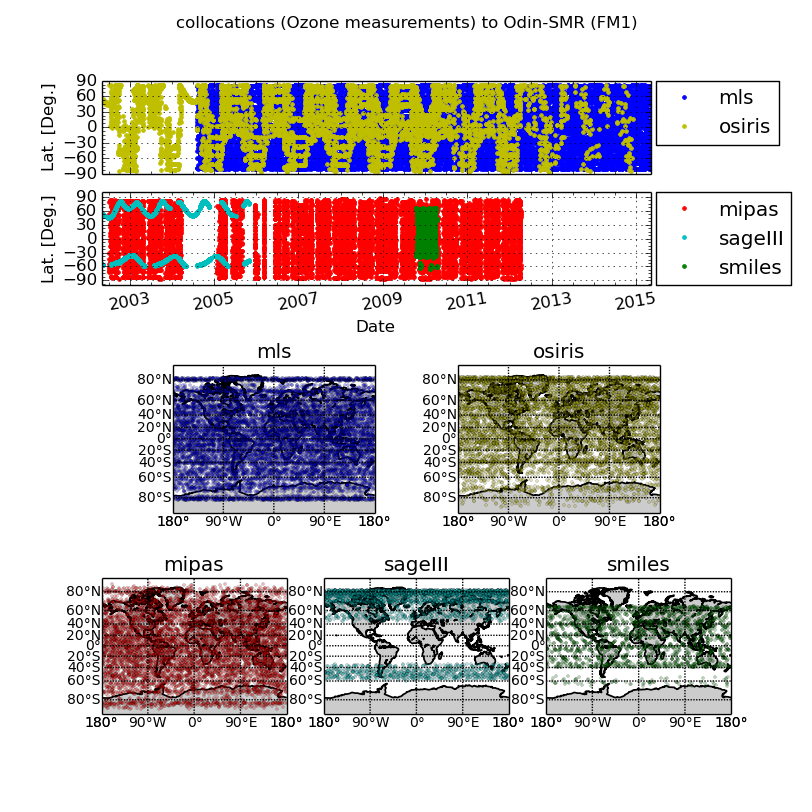
\includegraphics[width=17cm]{test_collocation_fm1.png}
\caption{VDS:Positions of collocated scans for frequency mode 1.}
\label{fig:vdsfm1}
\end{figure}



The VDS consists of a selected subset of the \smr\ dataset, and correlative
datasets to be used for validation purposes. 
The VDS should ideally include \smr\ measurements from    
the complete mission and for all geopraphical regions.
The VDS can be seen as a dataset of \smr\ measurements and
collocated measurements from the instrument described 
in the preceeding section. In this section we describe
how the VDS was selected.

 
Two measurements are considered to be collocated if they
are close in time and space. As a baseline for this VDS,
two measurements are considered to be collocated if the 
difference in distance and observation time between two profiles are 
less than 300\,km and and 1\,h, respectively.

However, a problem with this "strict" time difference criteria
is that collocations between \smr\ and  ENVISAT/MIPAS and Aura/MLS
are only found for high latitudes (around 80\,\degree\ N and around 80\,\degree\ S),
due to the fact each of these platform follows a sun-synchronous orbit
with quite different ascending equator crossing local times  
(18:00 hour for \smr\, 10:00 hour for ENVISAT/MIPAS,
 13:45 hour for Aura/MLS).
The VDS should ideally cover \smr\ measurements from    
the complete mission and all latitudes. 
Thus, for low latitudes the time difference criteria
is relaxed to 6\,hour for ENVISAT/MIPAS and Aura/MLS.
This gives effectively that collocated ENVISAT/MIPAS and Aura/MLS 
measurements can be found for almost all \smr\ measurements, and a strategy
to reduce the size of the VDS must be applied.

The construction of the VDS is done in the following way (considering ENVISAT/MIPAS and Aura/MLS):
For each \smr\ observation mode and month, five collocated scans
(five for ENVISAT/MIPAS and five for Aura/MLS)  
are selected, within each 10\degree\ latitude bin
(85\degree\ N -- 75\degree\ N , 75\degree\ N -- 65\degree\ N, ... , 75\degree\ S -- 85\degree\ S),
to be included in the VDS. For the two outer latitude bins the
time difference criteria is 1\,h, while set to 6\,h for the other bins.  
Figure~\ref{fig:vdsfm1} shows a graphical view of the position in
time and space for the measurements included in the VDS for
frequency mode 1 of \smr.   





\section{Data format}




